\section{Technical Approach}

We began by building a simulator for general $M$-$N$-$K$ games.
We started with a very simple agent \texttt{RandomAgent} -- which simply gathered the set of legal moves and chose randomly between them.
This agent allowed us to test the simulator and would become the backbone of our next agent -- \texttt{SearchAgent}.

\subsection{Search-based Agents}

\textbf{The \texttt{SearchAgent}} uses a search algorithm that resembles Monte Carlo Tree Search (MCTS), which we call Nearly MCTS (NMCTS).
Chaslot et al. wrote a paper about MCTS and its usefulness for solving board games of the modern and classic variety, as well as even video games~\cite{chaslot2008monte}.
Given a board at timestep $t$, the agent again collects the set of legal moves and then performs 1 step of search by copying the board and ``imagining'' making each legal move -- generating a board at timestep $t+1$.
This board is then used by 2 \texttt{RandomAgent}s to compute a set number of random rollouts to a terminal state.
Using the set of wins/losses/draws from the random rollouts, the \texttt{SearchAgent} now has an estimate of the quality of the state that results from selecting each action.

\begin{algorithm}
\caption{SearchAgents::move(board)}
\begin{algorithmic}[1]
\STATE{estWins = []}
\STATE{estLosses = []}
\STATE{estDraws = []}
\FOR{($i$,$j$) in availSquares}
\STATE{wins = losses = draws = $0.0$}
\FOR{games in numGamestoEstimate}
\STATE{Create deep copy of board}
\STATE{Add piece to ($i$,$j$) in copy}
\STATE{Play random game from here}
\IF{Win game}
\STATE{wins $\leftarrow$ wins + 1}
\ELSIF{Lose game}
\STATE{losses $\leftarrow$ losses + 1}
\ELSE{}
\STATE{draws $\leftarrow$ draws + 1}
\ENDIF{}
\ENDFOR{}
\STATE{Append wins to estWins}
\STATE{Append losses to estLosses}
\STATE{Append draws to estDraws}
\ENDFOR{}
\STATE{MoveScores = $2 \times wins - losses + draws$ }
\RETURN{availSquares( argmax( moveScores ) )}
\end{algorithmic}

\end{algorithm}

\subsubsection{Search-based Action Selection}

However, given a 3-element tuple of wins/losses/draws, selecting an action is not so easy!
For example, we specified that the agent should select the \texttt{argmax\{ estimatedWin \}}, which resulted in a very aggressive agent that was singularly focused on forming its sequence and disregarded the other agent's actions.
This resulted in games where the agent would be second to act, but still choose to race its opponent rather than defend.

\begin{figure}
	\centering
	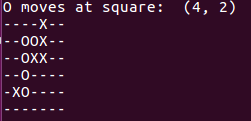
\includegraphics[ width = \columnwidth ]{Assets/argmax_9}
	\caption{A Sample of a Search-Based Agent's roll-outs as probabilities }
	\label{fig:argmax_1}
\end{figure}

So, we also varied our agent's approach to select the \texttt{argmin\{ estimatedLosses \}}, which led to a very defensive agent that usually played to a draw.
These agents were so focused on blocking any sequence of their enemy that they did not seem to want to form a sequence of their own.
To illustrate, we observed that when the agent was first to act, it would choose to defend its opponent rather than race to complete a sequence.
We hypothesized that some linear combinations of win, loss, and draw probabilities might make for a more effective agent, so we developed the equation:
\emph{Score = 2 * Win - Loss + Draw}
When we tested \texttt{argmax\{ Score \}}, we noticed that the behavior was almost identical to the \texttt{argmin\{ estimatedLosses \}}.

\subsection{The Neural Network Agent}

We wanted to compare the \texttt{SearchAgent} to one that uses a neural network to compete.
We call this agent the \texttt{nnAgent}, and its architecture follows that the input, the board, is passed through 
some convolutional layers, each with a 3x3 filter with padding.
Once the board has passed through these convolution layers, it is then passed through a fully connected layer with M * N outputs.
These output are then passed through two linear layers, the \emph{critic} and the \emph{actor}.
The critic takes the board size units and outputs one unit.
This estimates the value of the current state, under the assumption that the agent will behave according to the same policy in the future.
The actor, however, takes the board size (M * N) as input and has M * N outputs.
The actor selects the output unit that is most activated (via softmax), and that becomes the \texttt{nnAgent}'s move.

\begin{figure}
	\centering
	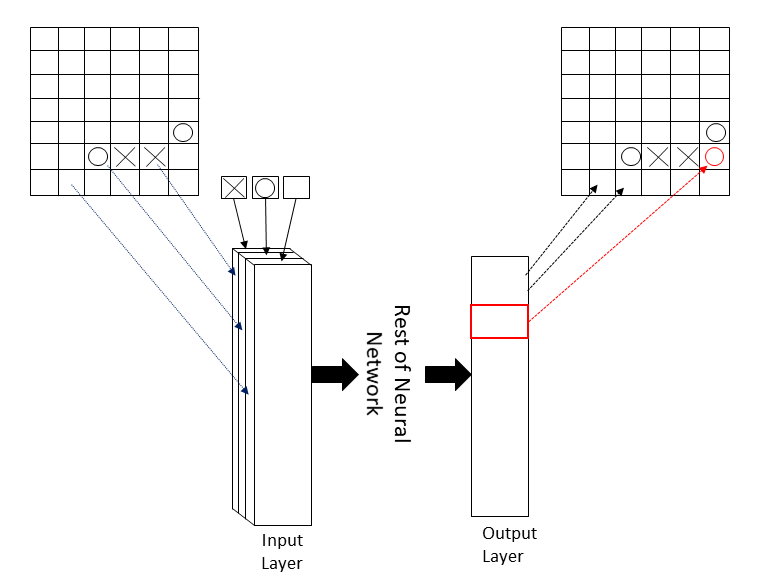
\includegraphics[width = \columnwidth, height = 70mm]{Assets/NetworkArchitecture3}
	\caption{The architecture of the CNN agent that plays, up until the actor/critic stage
    }
    \vspace{-4mm}
\label{fig:networkArchitecture}
\end{figure}

\begin{algorithm}
\caption{nnAgent(squareType, m, n, k)}
\begin{algorithmic}[1]
\STATE{nn.Conv2d(chans, c1Outs, kern, pad=int(kern/2))}
\STATE{nn.Conv2d(c1Outs, c2Outs, kern, pad=int(kern/2))}
\STATE{nn.Linear(c2Outs * m * n, m * n)}

\STATE{actor = nn.Linear(m * n, m * n)}
\STATE{critic = nn.Linear(m * n, 1)}
\end{algorithmic}

\end{algorithm}

\subsubsection{Training, Rewards, and Targets}

We used reinforcement learning to train the network.
If an agent tries to make an invalid move, such as trying to lay their glyph over an occupied spot, then a strong negative reward is given immediately.
In addition, the agent performs a weight update and is given another chance to make a legal move (up to a fixed number of tries, currently set at 300).
If the number of tries is exceeded, the agent reports the illegal move provided by the network, and the simulator will ignore it.
In essence, if the network fails to provide a legal move in a good number of tries, it loses its turn.

Once a game is complete, a reward is obtained.
A positive reward is obtained for the agent that wins, and a negative reward is obtained for the agent that loses.
If there is a draw, there is a smaller positive reward given to both agents.
Using this reward, we generate a target by taking a forward step, capturing the NN outputs, using them to determine the selected action, then modifying the target activation level \emph{for ONLY that action} by adding the reward to it.
The target values for the non-selected actions remains the same as the NN's output.
Thus, there is always loss in the network, because when the agent observes positive, pulling the target activation down will serve to reduce the probability that action is selected (and vice versa for negative reward).
The loss function we used was the Smooth-L1 loss, which is also known as least absolute errors.
It takes an output and target which are the same shape, which is ideal for our circumstances, where the lack of a ``true label'' rules out using something like cross entropy.

\begin{algorithm}
\caption{nnAgent::observeReward(history, reward)}
\begin{algorithmic}[1]
\STATE{Create Optimizer}
\STATE{Split history into just boards}
\FOR{board in history}
\STATE{nnOutput = forwardPass(board)}
\STATE{actionIdx = argmax(softmax(nnOutput))}
\STATE{target = nnOutput}
\STATE{target[actionIdx] += reward}
\STATE{loss = SmothL1Loss()(nnOutput, target)}
\STATE{backwardPass and update weights}
\ENDFOR{}
\end{algorithmic}

\end{algorithm}

\subsubsection{Stabilizing the Gradient}

Since our approach does not use any kind of memory replay (as done in~\cite{pytorchTut}), our gradient estimations can be very noisy.
One of the main extensions that would benefit our project is implementing a batch-mode gradient update using uncorrelated samples.
Currently, we are updating using the gradient from 1 complete action history, which is correlated.
We would like to store a database of the agent's experiences anyway, since querying it could be useful for explanation, in addition to improving gradient estimation. 
Our network uses the Adam optimizer with a learning rate of 1e-3 and a weight decay of 1e-4.